\section{Auswertung}
\label{sec:Auswertung}

\subsection{Bragg-Bedingung}
\label{sec:Bragg}

Die Messwerte zur Überprüfung der Bragg-Bedingung sind in \autoref{tab:Bragg} zu finden und in \autoref{fig:bragg}
dargestellt. Es wurde ein Maxium bei $27,7^{\circ}$ festgestellt. Nachdem Reflexionsgesetz liegt der
theoretische Winkel bei $28^{\circ}$. Daraus ergibt sich eine Abweichung von $1,5\%$.

\begin{table}
  \centering
  \begin{tabular}{c c | c c}
    \toprule
    $\theta^{\circ}$ & $N/Imp/s$ & $\theta^{\circ}$ & $N/Imp/s$ \\
    \midrule
    26,0 &  39,0 & 28,2 & 272,0 \\
    26,1 &  43,0 & 28,3 & 263,0 \\
    26,2 &  43,0 & 28,4 & 255,0 \\
    26,3 &  52,0 & 28,5 & 247,0 \\
    26,4 &  76,0 & 28,6 & 234,0 \\
    26,5 &  85,0 & 28,7 & 236,0 \\
    26,6 & 113,0 & 28,8 & 222,0 \\
    26,7 & 117,0 & 28,9 & 206,0 \\
    26,8 & 146,0 & 29,0 & 181,0 \\
    26,9 & 164,0 & 29,1 & 185,0 \\
    27,0 & 183,0 & 29,2 & 164,0 \\
    27,1 & 182,0 & 29,3 & 155,0 \\
    27,2 & 216,0 & 29,4 & 154,0 \\
    27,3 & 219,0 & 29,5 & 129,0 \\
    27,4 & 238,0 & 29,6 & 110,0 \\
    27,5 & 256,0 & 29,7 & 100,0 \\
    27,6 & 281,0 & 29,8 &  90,0 \\
    27,7 & 277,0 & 29,9 &  84,0 \\
    27,8 & 274,0 & 30,0 &  75,0 \\
    27,9 & 269,0 & & \\
    28,0 & 278,0 & & \\
    28,1 & 274,0 & & \\
    \bottomrule
  \end{tabular}
  \caption{Messwerte zur Überrüfung der Bragg-Bedingung.}
  \label{tab:Bragg}
\end{table}

\begin{figure}
  \centering
  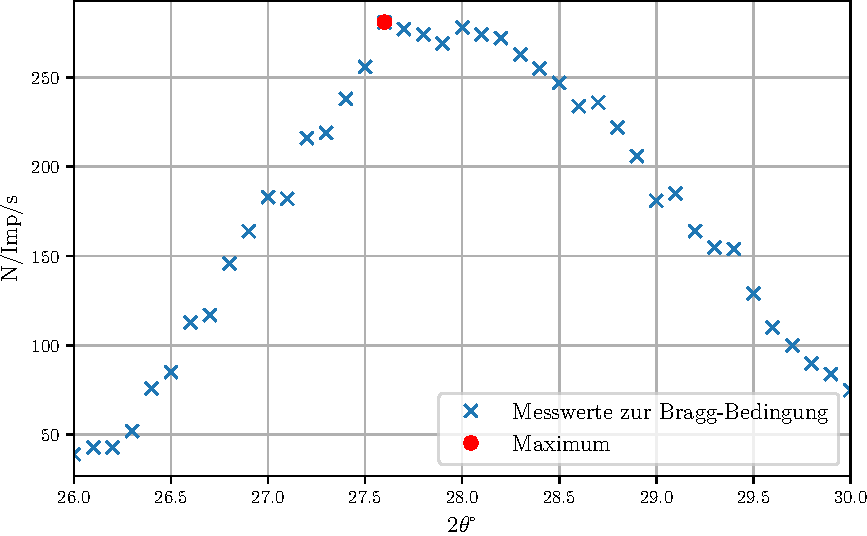
\includegraphics{bragg.pdf}
  \caption{Werte zur Bestimmung der Bragg-Bedingung.}
  \label{fig:bragg}
\end{figure}

\subsection{Emissionsspektrum der Cu-Röntgenröhre}
\label{sec:cu}

Die Messwerte der Kupferröntgenröhre sind in xxxxxxx zu finden.

\begin{table}
  \centering
  \begin{tabular}{c c | c c}
    \toprule
    $\theta^{\circ}$ & $N/Imp/s$ & $\theta^{\circ}$ & $N/Imp/s$ \\
    \midrule
     4.0 &  40.0 & 15.2 &  247.0 \\
     4.2 &  42.0 & 15.4 &  244.0 \\
     4.4 &  38.0 & 15.6 &  237.0 \\
     4.6 &  34.0 & 15.8 &  244.0 \\
     4.8 &  37.0 & 16.0 &  224.0 \\
     5.0 &  60.0 & 16.2 &  221.0 \\
     5.2 &  70.0 & 16.4 &  224.0 \\
     5.4 & 113.0 & 16.6 &  218.0 \\
     5.6 & 130.0 & 16.8 &  203.0 \\
     5.8 & 144.0 & 17.0 &  197.0 \\
     6.0 & 167.0 & 17.2 &  200.0 \\
     6.2 & 189.0 & 17.4 &  196.0 \\
     6.4 & 201.0 & 17.6 &  188.0 \\
     6.6 & 221.0 & 17.8 &  186.0 \\
     6.8 & 238.0 & 18.0 &  170.0 \\
     7.0 & 273.0 & 18.2 &  174.0 \\
     7.2 & 279.0 & 18.4 &  165.0 \\
     7.4 & 299.0 & 18.6 &  176.0 \\
     7.6 & 296.0 & 18.8 &  158.0 \\
     7.8 & 304.0 & 19.0 &  161.0 \\
     8.0 & 329.0 & 19.2 &  154.0 \\
     8.2 & 335.0 & 19.4 &  152.0 \\
     8.4 & 333.0 & 19.6 &  150.0 \\
     8.6 & 351.0 & 19.8 &  200.0 \\
     8.8 & 366.0 & 20.0 & 1374.0 \\
     9.0 & 377.0 & 20.2 & 1437.0 \\
     9.2 & 375.0 & 20.4 & 1021.0 \\
     9.4 & 385.0 & 20.6 &  230.0 \\
     9.6 & 376.0 & 20.8 &  205.0 \\
     9.8 & 395.0 & 21.0 &  185.0 \\
    10.0 & 414.0 & 21.2 &  177.0 \\
    10.2 & 416.0 & 21.4 &  169.0 \\
    10.4 & 408.0 & 21.6 &  179.0 \\
    10.6 & 417.0 & 21.8 &  194.0 \\
    10.8 & 403.0 & 22.0 &  269.0 \\
    11.0 & 424.0 & 22.2 & 2417.0 \\
    11.2 & 409.0 & 22.4 & 4662.0 \\
    11.4 & 411.0 & 22.6 & 4345.0 \\
    11.6 & 403.0 & 22.8 & 1292.0 \\
    11.8 & 393.0 & 23.0 &  182.0 \\
    12.0 & 381.0 & 23.2 &  142.0 \\
    12.2 & 385.0 & 23.4 &  124.0 \\
    12.4 & 389.0 & 23.6 &  114.0 \\
    12.6 & 389.0 & 23.8 &  109.0 \\
    12.8 & 374.0 & 24.0 &  104.0 \\
    13.0 & 370.0 & 24.2 &  103.0 \\
    13.2 & 351.0 & 24.4 &   91.0 \\
    13.4 & 322.0 & 24.6 &   87.0 \\
    13.6 & 294.0 & 24.8 &   91.0 \\
    13.8 & 277.0 & 25.0 &   84.0 \\
    14.0 & 273.0 & 25.2 &   81.0 \\
    14.2 & 270.0 & 25.4 &   77.0 \\
    14.4 & 263.0 & 25.6 &   78.0 \\
    14.6 & 261.0 & 25.8 &   76.0 \\
    14.8 & 244.0 & 26.0 &   79.0 \\
    15.0 & 250.0 & & \\
    \bottomrule
  \end{tabular}
  \caption{Messwerte der Kupferröntgenröhre.}
\end{table}

\begin{figure}
  \centering
  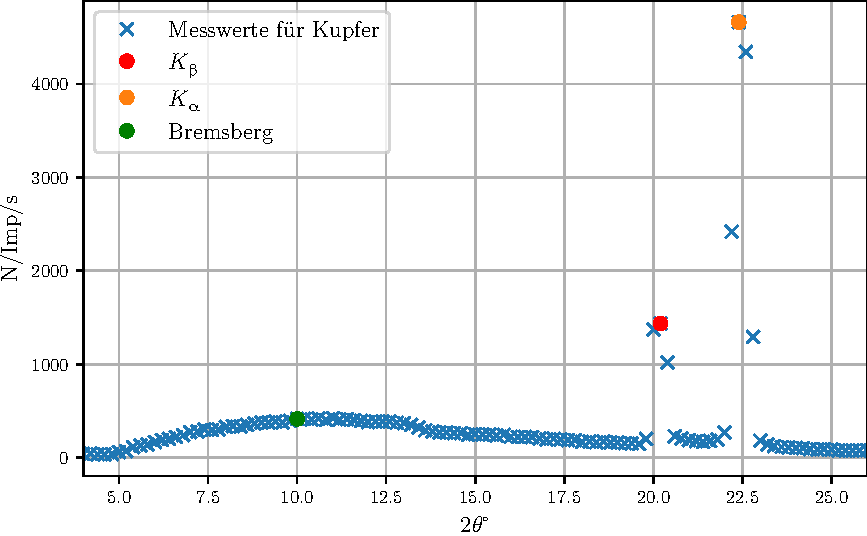
\includegraphics{cu.pdf}
  \caption{Emissionsspektrum der Cu-Röntgenröhre.}
  \label{fig:cu}
\end{figure}